% ============================================================
\chapter{Wave Equation}
\label{ch:wave}
% ============================================================

Pluck a guitar string. The perturbation travels in both directions, bounces off the endpoints, and produces a sound whose frequency depends on the length, tension, and linear density of the string. The wave equation, formulated by d'Alembert in 1747 for the vibrating string, is the first PDE ever written. Unlike the heat equation, it is time-reversible: waves do not dissipate, they propagate at finite speed and preserve their shape. D'Alembert's solution in one dimension shows that every solution is a superposition of two waves travelling in opposite directions---an observation of remarkable simplicity and power.

\section{Physical motivation}

The wave equation describes the propagation of perturbations through a
medium: vibrations of a string or membrane, sound waves, electromagnetic
waves. Unlike the heat equation, propagation occurs at \textbf{finite speed}
and without dissipation.

\begin{definition}[Wave equation]
The \textbf{wave equation} in dimension $n$ is:
\begin{equation}\label{eq:wave}
    u_{tt} - c^2 \Delta u = f(x,t), \quad x \in \R^n,\; t > 0,
\end{equation}
where $c > 0$ is the propagation speed.
\end{definition}

\section{Wave equation in dimension 1}

\subsection{d'Alembert's formula}

\begin{theorem}[d'Alembert's formula]
The solution of the Cauchy problem:
\begin{equation}\label{eq:cauchy_wave_1d}
    \begin{cases}
        u_{tt} = c^2 u_{xx}, & x \in \R,\; t > 0,\\
        u(x,0) = g(x), \quad u_t(x,0) = h(x),
    \end{cases}
\end{equation}
is given by \textbf{d'Alembert's formula}:
\begin{equation}\label{eq:dalembert}
    \boxed{u(x,t) = \frac{g(x+ct) + g(x-ct)}{2}
    + \frac{1}{2c}\int_{x-ct}^{x+ct} h(s)\, ds.}
\end{equation}
\end{theorem}

\begin{proof}
We introduce \textbf{characteristic coordinates} $\xi = x + ct$,
$\eta = x - ct$. The equation $u_{tt} = c^2 u_{xx}$ becomes
$u_{\xi\eta} = 0$, whose general solution is:
\[
    u(\xi, \eta) = F(\xi) + G(\eta) = F(x+ct) + G(x-ct),
\]
where $F$ and $G$ are arbitrary functions. The initial conditions give:
\[
    F(x) + G(x) = g(x), \quad c\, F'(x) - c\, G'(x) = h(x).
\]
Integrating the second equation and solving the system yields d'Alembert's
formula.
\end{proof}

\begin{center}
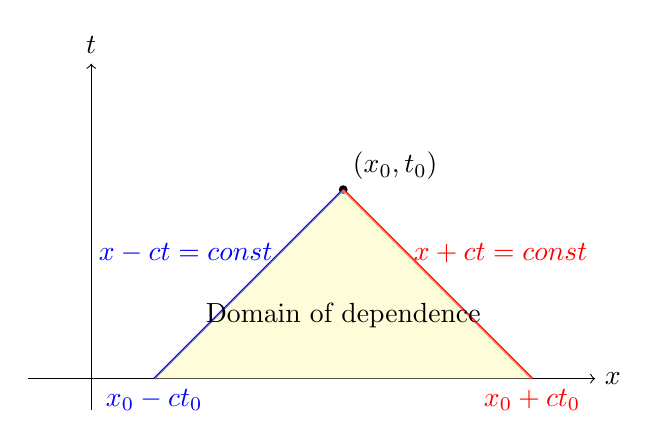
\begin{tikzpicture}[scale=0.8]
    \draw[->] (-1,0) -- (8,0) node[right] {$x$};
    \draw[->] (0,-0.5) -- (0,5) node[above] {$t$};
    % Point
    \fill (4,3) circle (2pt) node[above right] {$(x_0, t_0)$};
    % Characteristics
    \draw[blue, thick] (4,3) -- (1,0) node[below] {$x_0-ct_0$};
    \draw[red, thick] (4,3) -- (7,0) node[below] {$x_0+ct_0$};
    % Domain of dependence
    \fill[yellow!30, opacity=0.5] (4,3) -- (1,0) -- (7,0) -- cycle;
    \node at (4, 1) {Domain of dependence};
    % Labels
    \node[blue] at (1.5, 2) {$x-ct=\text{const}$};
    \node[red] at (6.5, 2) {$x+ct=\text{const}$};
\end{tikzpicture}
\end{center}

\begin{keyformulas}[title=\textbf{1D wave equation --- key formulas}]
\begin{itemize}
    \item d'Alembert: $u = \frac{1}{2}[g(x+ct)+g(x-ct)] + \frac{1}{2c}\int_{x-ct}^{x+ct} h(s)\, ds$.
    \item Characteristics: $x \pm ct = \text{const}$.
    \item General solution: $u = F(x+ct) + G(x-ct)$.
\end{itemize}
\end{keyformulas}

\subsection{Domain of dependence and influence}

\begin{definition}[Domain of dependence]
The \textbf{domain of dependence} of the point $(x_0, t_0)$ is the
interval $[x_0 - ct_0, x_0 + ct_0]$ on the axis $t = 0$. The solution
at $(x_0, t_0)$ depends only on the initial data on this interval.
\end{definition}

\begin{definition}[Domain of influence]
The \textbf{domain of influence} of the point $x_0$ on the axis $t = 0$ is
the cone $\{(x,t) : \abs{x - x_0} \leq ct,\; t > 0\}$.
\end{definition}

\begin{theorem}[Finite speed of propagation]
If the initial data $g$ and $h$ are supported in $[a,b]$, then
$u(x,t) = 0$ for $x \notin [a-ct, b+ct]$. Information propagates at
most at speed $c$.
\end{theorem}

\section{Energy conservation}

\begin{theorem}[Energy conservation]
If $u$ solves $u_{tt} = c^2\Delta u$ in $\R^n$, the \textbf{energy}:
\begin{equation}\label{eq:wave_energy}
    E(t) = \frac{1}{2}\int_{\R^n}
    \left(u_t^2 + c^2\abs{\nabla u}^2\right) dx
\end{equation}
is conserved: $E(t) = E(0)$ for all $t \geq 0$.
\end{theorem}

\begin{proof}
We compute:
\begin{align*}
    E'(t) &= \int_{\R^n} \left(u_t\, u_{tt} + c^2 \nabla u \cdot \nabla u_t\right) dx \\
    &= \int_{\R^n} u_t \left(u_{tt} - c^2\Delta u\right) dx = 0.
\end{align*}
The last equality uses integration by parts
($\int \nabla u \cdot \nabla u_t = -\int u_t\, \Delta u$).
\end{proof}

\begin{corollary}[Uniqueness]
The Cauchy problem for the wave equation admits at most one solution
(in a suitable regularity class).
\end{corollary}

\section{Vibrating string with fixed endpoints}

\begin{example}
Solve:
\[
    \begin{cases}
        u_{tt} = c^2 u_{xx}, & 0 < x < L,\; t > 0,\\
        u(0,t) = u(L,t) = 0,\\
        u(x,0) = g(x), \quad u_t(x,0) = h(x).
    \end{cases}
\]
By separation of variables:
\[
    u(x,t) = \sum_{n=1}^{\infty} \sin\!\left(\frac{n\pi x}{L}\right)
    \left[A_n \cos(\omega_n t) + B_n \sin(\omega_n t)\right],
\]
with $\omega_n = \frac{cn\pi}{L}$ (natural frequencies). The coefficients are:
\[
    A_n = \frac{2}{L}\int_0^L g(x)\sin\!\left(\frac{n\pi x}{L}\right) dx,
    \quad
    B_n = \frac{2}{L\omega_n}\int_0^L h(x)\sin\!\left(\frac{n\pi x}{L}\right) dx.
\]

The solution is a superposition of \textbf{normal modes} vibrating at
frequencies $\omega_n = cn\pi/L$. The fundamental frequency is
$\omega_1 = c\pi/L$; the others are \textbf{harmonics}
$\omega_n = n\omega_1$.
\end{example}

\begin{intuition}
Each normal mode $\sin(n\pi x/L)\cos(\omega_n t)$ represents a
\textbf{standing wave}: the spatial shape remains fixed and only the
amplitude oscillates. The superposition of modes produces the complex
shapes of a vibrating string.
\end{intuition}

\section{Wave equation in higher dimensions}

\subsection{Dimension 3: Kirchhoff's formula}

\begin{theorem}[Kirchhoff's formula]
The solution of the Cauchy problem in dimension 3:
\[
    u_{tt} = c^2 \Delta u, \quad u(x,0) = g(x), \quad u_t(x,0) = h(x),
\]
is:
\begin{equation}\label{eq:kirchhoff}
    u(x,t) = \frac{1}{4\pi c^2 t}\iint_{S(x,ct)} h(y)\, dS(y)
    + \frac{\partial}{\partial t}\left[\frac{1}{4\pi c^2 t}
    \iint_{S(x,ct)} g(y)\, dS(y)\right],
\end{equation}
where $S(x,ct)$ is the sphere centred at $x$ with radius $ct$.
\end{theorem}

\begin{theorem}[Strong Huygens' principle]
In dimension $n = 3$ (and more generally for odd $n \geq 3$), the
\textbf{strong Huygens' principle} holds: the solution at $(x,t)$
depends only on the data on the sphere $\abs{y-x} = ct$, not in the ball.
Physically, a point signal produces a sharp wavefront that passes and
vanishes.
\end{theorem}

\subsection{Dimension 2: Poisson's formula}

\begin{theorem}[Poisson's formula --- dimension 2]
In dimension 2, the solution is:
\begin{equation}\label{eq:poisson_wave_2d}
    u(x,t) = \frac{1}{2\pi c}\iint_{B(x,ct)}
    \frac{h(y)}{\sqrt{c^2 t^2 - \abs{y-x}^2}}\, dy
    + \frac{\partial}{\partial t}\left[\frac{1}{2\pi c}\iint_{B(x,ct)}
    \frac{g(y)}{\sqrt{c^2 t^2 - \abs{y-x}^2}}\, dy\right].
\end{equation}
\end{theorem}

\begin{warning}[title=\textbf{No Huygens' principle in even dimensions}]
In dimension 2, the solution depends on data in the entire disk $B(x,ct)$,
not just on the circle. This is why waves on water leave a wake behind
them (unlike sound waves in 3D).
\end{warning}

\section{Damped wave equation}

The damped wave equation reads:
\[
    u_{tt} + 2\gamma u_t = c^2 \Delta u, \quad \gamma > 0.
\]
The term $2\gamma u_t$ models friction proportional to velocity.

\begin{proposition}[Energy decay]
For the damped equation, the energy decreases:
\[
    E'(t) = -2\gamma \int_{\R^n} u_t^2\, dx \leq 0.
\]
\end{proposition}

\section{Exercises}

\begin{exercise}
Use d'Alembert's formula to solve $u_{tt} = u_{xx}$ with
$u(x,0) = e^{-x^2}$ and $u_t(x,0) = 0$. Sketch the solution for
$t = 0, 1, 2$.
\end{exercise}

\begin{exercise}
Solve $u_{tt} = 4u_{xx}$ with $u(x,0) = 0$ and
$u_t(x,0) = \mathbf{1}_{[-1,1]}(x)$. Determine the domain of dependence
and sketch the solution.
\end{exercise}

\begin{exercise}
Vibrating string: solve $u_{tt} = u_{xx}$ on $(0,\pi)$ with
$u(0,t) = u(\pi,t) = 0$, $u(x,0) = \sin(x)\sin(2x)$, $u_t(x,0) = 0$.
\end{exercise}

\begin{exercise}
Show that energy conservation implies uniqueness for the Cauchy problem.
\end{exercise}

\begin{exercise}[Reflection at a fixed boundary]
Let $u_{tt} = c^2 u_{xx}$ for $x > 0$, $t > 0$ with $u(0,t) = 0$ and
initial data compactly supported in $(0,\infty)$. Use the method of images
(odd extension) to construct the solution.
\end{exercise}

\begin{exercise}
For the damped wave equation $u_{tt} + 2\gamma u_t = c^2 u_{xx}$, show
that $E(t) \leq E(0)\, e^{-2\gamma t}$.
\end{exercise}

\begin{exercise}
Verify Kirchhoff's formula in 3D for the case $g = 0$, $h(x) = 1$
(constant data). Find $u(0,t)$ explicitly.
\end{exercise}

\begin{exercise}[Duhamel's principle for the wave equation]
Show that the solution of $u_{tt} - c^2 u_{xx} = f(x,t)$ with
$u(x,0) = u_t(x,0) = 0$ is:
\[
    u(x,t) = \frac{1}{2c}\int_0^t \int_{x-c(t-s)}^{x+c(t-s)} f(y,s)\, dy\, ds.
\]
\end{exercise}
